\chapter{Przegląd metod detekcji i~identyfikacji obiektów w~obrazach}

W~tym rozdziale przedstawione zostaną algorytmy detekcji (wykrywania,
lokalizacji) obiektów w~obrazach, oraz ich identyfikacji (rozpoznawania).
Wskazane zostaną obszary dobrze znane i~udokumentowane takie jak detekcja
twarzy, do obsługi których istnieją ogólnodostępne implementacje
rozwiązujące problem na zadowalającym poziomie. Z~drugiej strony
przedstawione zostaną dziedziny w~zakresie których prowadzone są intensywne
badania m.in. odczytywanie tekstu ze sceny, gdzie nie istnieje uniwersalne
rozwiązanie.

Na potrzeby tego opracowania wprowadzone zostaną dwa terminy. Zgodnie
z~tytułem rozdziału, będzie to detekcja obiektów, oraz identyfikacja
obiektów. Pod pojęciem detekcji kryje się proces wykrywania obiektów
pewnej klasy w~zadanym obrazie wejściowym. 
Wynikiem działania algorytmu detekcji jest zazwyczaj lista
współrzędnych określających położenie obiektu w~obrazie - prostokąty
okalające. Dobrze zbadane dziedziny wykrywania obiektów to m.in. 
wykrywanie twarzy czy wykrywanie przechodniów. Do omawianej dziedziny
zalicza się również lokalizacja tekstu w~scenie, gdzie podzbiorem
tego zagadnienia jest wykrywanie i~lokalizacja numerów.

Kolejnym zagadnieniem jest rozpoznawanie obiektów. Różnica między
detekcją, a~identyfikacją na przykładzie twarzy wygląda następująco.
Detektor twarzy lokalizuje wszystkie wystąpienia obiektów danej klasy
w~scenie - może nie zwrócić nic, gdy fotografowana była na przykład martwa
natura. ,,Identyfikator'' twarzy uruchamiany jest dla każdego wystąpienia
twarzy w~scenie i~zwraca informację do kogo dana twarz należy.
Identyfikacja lub inaczej rozpoznawanie obiektów jest zadaniem z~założenia
bardziej złożonym, zarówno koncepcyjnie jak i~obliczeniowo.
Przykładowe zastosowania algorytmów rozpoznawania obiektów to wspomniane
już identyfikowanie osoby na podstawie twarzy, którego wariantem może
być identyfikowanie osoby na podstawie siatkówki oka lub odcisku palca,
w~których to przypadkach element wykrywania jest pominięty. 
Pewną parafrazą
rozpoznawania obiektów jest identyfikacja znaków w~algorytmach odczytywania
tekstu (\textit{ang. OCR - Optical Character Recognition}).

Logiczny podział algorytmów i~ich implementacji jest zadaniem 
wykraczającej poza zakres tego opracowania. Niektóre rozwiązania
zaprojektowane do wykrywania po trywialnych modyfikacjach mogą służyć
do rozpoznawania wykrytych obiektów. Ostatecznie niektóre detektory
w~efekcie ubocznym mogą służyć do identyfikacji znalezionych obiektów.

\section{Wykrywanie obiektów A.K.A. detekcja}

Na potrzeby pracy wprowadzony i~opisany został termin 
,,detekcji obiektów''. Na wejściu tak zdefiniowanego detektora
jest obraz zawierający (lub nie) wystąpienia interesujących obiektów, gdzie
wyjściem jest lista przyciętych obrazów reprezentujących wystąpienia tych
obiektów (fizyczne kopie lub współrzędne).

Poniżej przedstawione zostały rozwiązania nawiązujące do powyższego opisu.

\subsection{Kaskadowy Klasyfikator OpenCV}

Biblioteka OpenCV zawiera funkcje oraz całe środowisko do przygotowywania
i~używania kaskodowych detektorów różnych typów. W~dokumentacji
\cite{OCV:cascadeclassification}
jest mowa o~dwuch opracowaniach \cite{DBLP:conf/cvpr/ViolaJ01,
DBLP:conf/icip/LienhartM02} na których bazuje oferowana
implementacja.

Podstawowa funkcjonalność dostarczana przez implementację została zawarta
w~funkcji \verb|detectMultiScale|. Dla przekazanego obrazu (argument wywołania)
zwracana jest kolekcja reprezentująca wystąpienia szukanego obiektu.

Aby jednak skorzystać ze~wspomnianej funkcji trzeba przygotować plik
definiujący klasyfikator. Jest to proces żmudny o~tyle, iż wymaga relatywnie
dużej liczby oznaczonych wystąpień szukanych obiektów. Należy dostarczyć
tym dłuższą listę im większe zrużnicowanie w~obiektach reprezentujących
daną klasę. Prekursorzy rozwiązania - panowie Viola i Jones - mówią
o~danych wejściowych idących w~dziesiątki tysięcy. Internetowe źródła
mówią ilości pozytywnych przypadków rzędu 10-50 tysięcy, przy czym
negatywne przypadki (obrazy nie zawierające wystąpienia szykanych obiektów)
powinny stanowić nieco ponad połowę tego zbioru.

Kolejnym czynnikiem jest czas potrzebny na wyszkolenie detektora
(przygotowanie pliku). Pierwotna metoda oparta na cechach Haara
jest najbardziej intensywna obliczeniowo, a~cały proces uczenia
może trwać do kilku dni. Rozwiązania oparte na innych cechach - LBP
(\textit{ang. Local Binary Pattern}) - trwają stosunkowo krócej, lecz
nadal czas wykonania liczony jest w~godzinach.

Samo wyszukiwanie obiektów oparte jest na oknie przesuwnym
(\textit{ang. sliding window}). Wspomniane okno przemieszcza się nad
obrazem definiując kombinację podobrazów, dla których po koleji uruchamiany
jest algorytm określający czy dany fragment reprezentuje szukany obiekt czy
nie. Ograniczeniem wprowadzonym przez to podejscie jest brak możliwości
wykrycia obrotu, gdyż krawędzie okna są zawsze równoległe z~krawędziami
obrazu. Zaletą jest niewielka złożoność obliczeniowa, która pozwala
na wykrywanie i~lokalizowanie obiektów w~czasie rzeczywistym.

\subsection{Cechy 2D - Framework biblioteki OpenCV}

Biblioteka OpenCV poza wspomnianym detektorem udostępnia też cały
framework do operacji na cechach: wyliczanie, opisywanie i~dopasowywanie.
Tutaj w~odrużnieniu od detektora kaskadowego, zestaw cech
jest wyliczany dla każdego obrazu osobno i~jest to proces dużo bardziej
intensywny obliczeniowo niż w~poprzednim przypadku. Dodatkowo
funkcjonalność detekcji obiektów jest raczej efektem ubocznym,
a~ze względu na jednostkowy charaktery wyszukiwanych obiektów rozwiązanie
bardziej nadaje się do weryfikacji i~rozpoznawania obiektów niż do
detekcji i~lokalizacji obiektów pewnej klasy.

Przykład zastosowania zaprezentowano na rysunku poniżej.

\begin{figure}[h!]
  \centering
    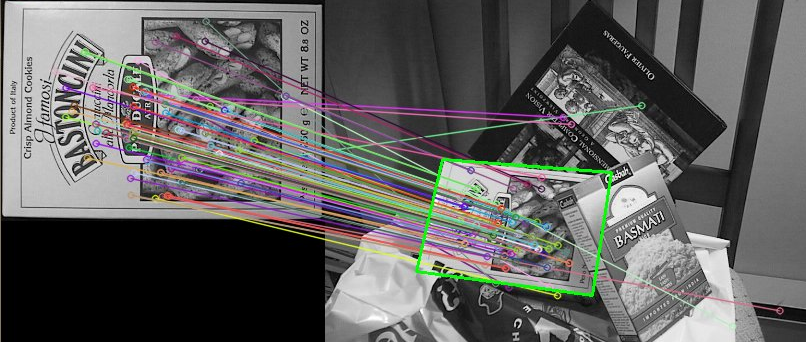
\includegraphics[width=0.8\textwidth]{img/rev_features2d_detection}
  \caption{Wykorzystanie framework-a cech 2d do wykrywania obiektów}
\end{figure}

Ze względu na mnogość zaimplementowanych algorytmów - których opis
wykracza poza zakres tego opracowania - istnieje ogromna ilość
zastosowań wspomnianego frameworka, w~tym detekcja obszarów
w~obrazach reprezentujących tekst w~scenach naturalnych. W~tym celu
można wykożystać implementację algorytmu MSER - (\textit{ang. Most
Stable Extreme Regions}).

\subsection{Open Track-Learn-Detect}

Ciekawostką w~dziedzinie detekcji obiektów jest algorytm opracowany przez
pana Zdenka Kalala \cite{DBLP:journals/pami/KalalMM12}.
Ograniczeniem jest potrzeba pierwszego oznaczenia wystąpienia interesującego
obiektu w~sekwencji obrazów tak aby algorytm mógł podjąć śledzenie.
Etap śledzenie jest połączony z~uczeniem detektora, który służy do wznowienia
śledzenia gdy obiekt zniknie z~kadru.

Dostępna jest implementacja w~języku C/C++ oraz MatLabie. W~trakcie
pisania tego tekstu pojawiła się druga wersja algorytmu niosąca
za sobą duże usprawnienia w~dziedzinie wydajności. Co zaprezentowano
na wykresie poniżej.

\begin{figure}[h!]
    \centering
    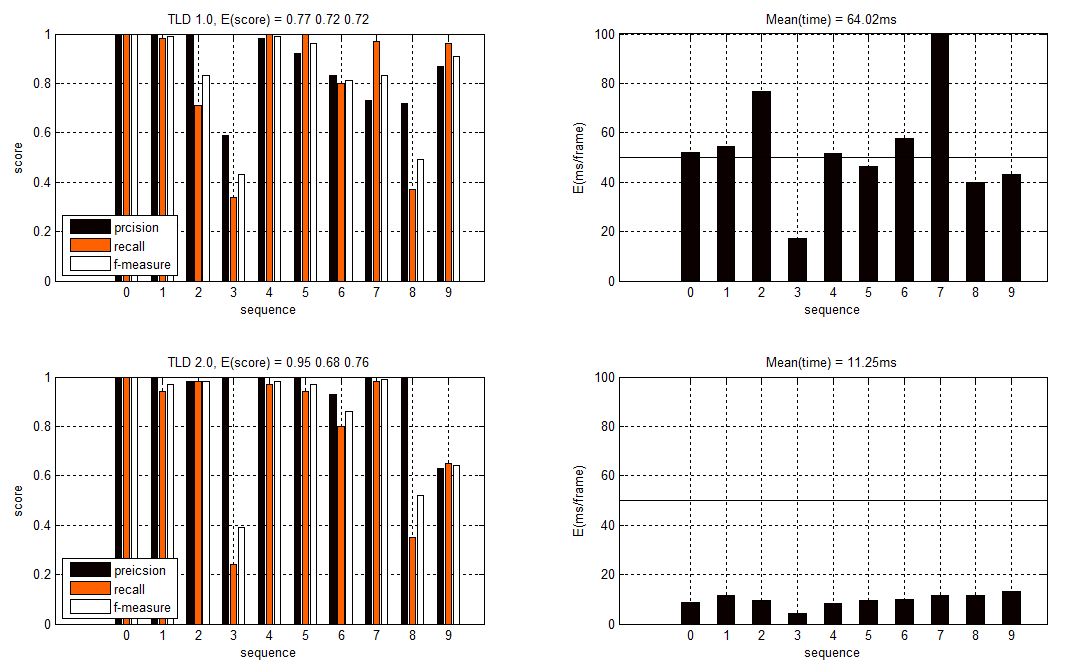
\includegraphics[width=1\textwidth]{img/rev_open_tld_1_2_comparison}
    \caption{Porównanie skuteczności i wydajności biblioteki OpenTLD w wersjach 1 i 2}
\end{figure}

Istnieje przypuszczenie, że pozostawienie algorytmu w~trybie uczenia
może powodować powoly spadek wydajności ze względu na rosnącą liczbę
pozytywnych i~negatywnych obiektów w~bazie. Jest to jednak teza wymagająca
przeprowadzenia żetelnych testów. Kolejnym utrudnieniem jest brak
prznaszalnej implementacji - dostępna jest tylko biblioteka skompilowana
dla systemu Windows.

\section{Rozpoznawanie obiektów A.K.A. identyfikacja}

Drugim terminem popza detekcją jest rozpoznawanie obiektów. Algorytm
identyfikacji najczęściej przyjmuje na wejściu obraz stałych rozmiarów
przedstawiający obiekt pewnej klasy. Zadaniem algorytmu jest zwrócenie
tekstu określającego typ, rodzaj lub po prostu nazwę danego obiektu.

Przykładem zastosowania może być odczytanie wykrytych liter,
cyfr, przypisanie twarzy do właścicieli lub zwrócenie marki wykrytego
samochodu.

Ze względu na specyfikę zagadnienia gotowych implementacji algorytmów
identyfikacji jest niewiele lub sprawdzają się one w~obrębie
ściśle okreśonego zagadnienia. Niektóre z~przytoczonych w~poprzednim
podrozdziale przykładów mogą równie dobrze służyć jako identyfikatory
obiektów. Algorytm OpenTLD skutecznie rozróżnia twarze, gesty oraz
poszczególne instancje obiektów różnych klas.

Klasycznym podejściem do identyfikacji jest uczenie maszynowe. Na
wejściu podowany jest zbiór reprezentantów poszczególnych klas
z~przypisanymi do nich oczekiwanymi rezultatami. Rozwiązanie
sprawdza się przy rozpoznawaniu znaków drukowanych o~wysokim
kontraście i~w~wysokiej rozdzielczości. Ograniczeniem jest bowiem
potrzeba wprowadzenia pojęcia odległości między poszczególnymy
reprezentantantami danej klasy. Wykorzystując do tego bibliotekę
OpenCV można wybrać dwie metody:

\begin{itemize}
\item K-średnich,
\item SVM.
\end{itemize}

Obie metody są podobne. Zakładają fazę uczenia i~rozpoznawania.
Jednak obliczanie odległości pomiędzy dwoma instancjami obiektu
i~wybór odpowiedniej metody ku temu pozostaje w~gestii programisty.
Niestety może to być dowolna metoda. Można użyć deskryptorów cech
SIFT, SURF, BRIEF itp. W~skrajnie laboratoryjnych warunkach, tak
jak w~odczytywaniu znaków czarno-białbych można porównywać poszczególne
piksele i~obliczać w~prost różnicę między obrazami. Jednak
jeżeli jednak tekst jest ulokowanany w~tak zwanej scenie naturalnej -
szyld, reklama, bilbord itp. - różnice w~czcionkach, refleksy
i~zniekształcenia uniemożliwiają wykorzystanie tak trywialnej metody.
Zagadnienie jest na tyle ważne i~jednocześnie skomplikowane, że
powstał plebiscyt, którego zadaniem jest wyłonienie najlepszego
algorytmu odczytującego teksty ze scen naturalnych. Odbywa się
on co dwa lata, a~ostatnia edycja miała miejsce w~roku 2013.
Zwycięzcy konkursu ICDAR2013 w~dziedzinie odczytywania tekstu ze
zdjęć, do rozpoznawania poszczególnych znaków wykorzystali sieci neuronowe.
Podobnie było w~przypadku algorytmu odczytującego numery domów na potrzeby
geolokalizacji w~usłudze google-street-view. Ostatecznie zadanie
odczytywania numerów/tekstów ze zdjęć jest zadaniem najtrudniejszym
z~dotąd omawianych.

\begin{figure}[h!]
    \centering
    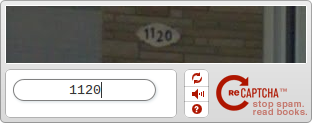
\includegraphics[width=0.8\textwidth]{img/rev_captcha_street_view}
    \caption{Przykładowa captcha z prawdopodobnym numerem domu}
\end{figure}

O~skali złożoności problemu może świadczyć fakt, iż
opracowany przez Google algorytm wymaga wspomagania w~postaci interwencji
białkowej. Przeglądając zasoby internetu napotkana została captcha
z~obrazkiem przypominającym numer domu, co może świadczyć, że stuprocentowa
automatyzacja rozpoznawania numerów domów nie do końca udała się inżynierom
z MountainView.

